\documentclass[12pt]{article}
\usepackage{newtxtext,newtxmath}
\usepackage[utf8]{inputenc}
\usepackage{amssymb}
\usepackage{mathtools}
\usepackage{gensymb}

\usepackage{caption}
\usepackage{subcaption}

\usepackage{hyperref}
\usepackage{xurl}
\usepackage[
backend=biber,
style=ieee,
]{biblatex}
\addbibresource{reference.bib}

\usepackage[a4paper, top=1.5cm, bottom=2.5cm, left=2.5cm, right=2.5cm]{geometry}
\newcommand{\floor}[1]{\lfloor #1 \rfloor}
\title{Thailand 2019 Election Analysis by Benford's Law}
\author{SHEN Junbo, ZHOU Yixiang, JARUTHIKORN Nutdranai (Group 11)}
\date{20 November 2021}

\begin{document}
\maketitle
\section{Abstract}

The distribution of the first digit of the numbers in a dataset is not always uniform, especially when it comes to real-life data. Described as Benford's Law, it appears that the leading digit is likely to be small if the dataset is intact from artificial modification. The concept of using the Law to monitor data corruption has been a well-established idea over the years, yet we have seen debate around the authenticity of the law being used as a weapon against potential frauds. In this project, we used some real-world data, namely the vote result from the latest Thailand Election, to show the capability and limitation of the much-anticipated law and learn how we can handle it more gracefully in data analysis.

\section{Introduction}

In many real life cases, the growth of some numbers is proportional to their current magnitude. The growth rate could be modelled by $\frac{\Delta f(t)}{\Delta t} = \text{constant}\times f(t)$, where $f(t)$ and $t$ denotes the generated value and time taken to reach $f(t)$. From this model, it could be proved \cite{yixiang} that the probability $P_i$ of the first digit of of $f(t)$ being $i$, over uniformly chosen $t$, is:
$$P_i = \log_{10}\frac{i+1}{i}$$
This is known as the \textbf{Benford's First Digit Law}, which could be generalised to a stronger version, \textbf{Benford's Law}, defined as follows. A random variable $X$ satisfies Benford's Law if $S(x)$ has a logarithmic distribution. In other words,
$$P(S(x) \leq t) = \log t, \quad t \in [1,10)$$where $S(x)$, is the significand function ($S(x) = 10^{ \{\log x\} }$). Since Benford's Law provides a distribution of the digits of a growing data set, it could use as a forensic tool detect fraudulent of real-life data \cite{walter}. To test a data set's compliance with Benford's Law, the chi-square goodness-of-fit statistic is recommended \cite{pike}, which is calculated by $$x_{calc}^2 = \sum_{i=1}^{9}\frac{(O_i - E_i)^2}{E_i}$$ where $O_i$ is the observed frequency of leading digit $i$ and $E_i$ is the expected frequency of leading digit $i$ according to Benford's Law. Here, \textbf{P-value}, the probability $P(X>x_{calc}^2)$, where $X$ is the chi-square random variable, is used as a criteria to the test. \newline \newline Recently, rumours have been circulating regarding transparency of \textbf{Thailand Election} in 2019. Furthermore, a report has been conducted reporting non-transparency in the election \cite{forsea}. Since it is shown that the election data must conform to Benford's Law \cite{walter}, we will use Benford's Law as a forensic tool to analyse the transparency of the Thailand Election Data set.


\section{Main Part}

\subsection{Data}
Thailand Election Data \cite{election} could be obtained from this \href{https://www.ect.go.th/ewt/ewt/ect_th/download/article/article_20190328165029.pdf}{\textbf{link}}. The data is in a spreadsheet format where each row represents a candidate of a particular party applying in a particular province and the votes him/her received. There were 77 parties involved.

\subsection{Data Processing}
The number of votes in each row of the spreadsheet is counted once to obtained the frequency of the leading digit of all the votes. Then, an analysis of the leading digit's frequency of each party is conducted. The calculation is done using the Jupyter notebook on Google Colab which could be found from \href{https://colab.research.google.com/drive/1Y7lz2Er4WxXexss0tcbCmE-tPEKGnbBs?usp=sharing}{\textbf{this link}}. We also have a GitHub repository which could be found from  \href{https://github.com/pond-nj/Benford-s-Law-Analysis}{\textbf{this link}} respectively.

\subsubsection* {Overall Data}
The leading digit frequency of every party is counted, and the graph (Figure 1a) is plotted with measured frequency (blue bars) and theoretical frequency (orange bars). It might be intuitively concluded that the count fits perfectly into the first digit law. Yet, this observation might not be statistically correct, which will be further elaborated later using chi-square and p-value analysis.

\subsubsection* {Party's Data}
The frequency of each party's vote is counted in the same way as the overall votes, which would be plotted and analysed using p-value and chi-square method. The graphs could be found in this \href{https://github.com/pond-nj/Benford-s-Law-Analysis/tree/main/thai\%20election\%20graph}{\textbf{folder}} on GitHub. We show the result of Palang Pracharat Party below as an example (Figure 1b).

\begin{figure}[h]
\centering
\begin{subfigure}{.5\textwidth}
  \centering
  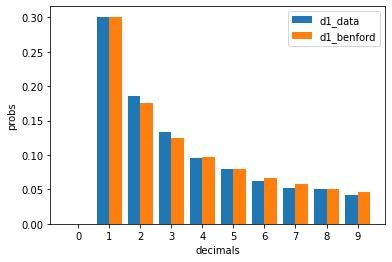
\includegraphics[scale=0.4]{complete thai analysis.png}
  \caption{First Digit Frequency of All votes}
  \label{fig:sub1}
\end{subfigure}%
\begin{subfigure}{.5\textwidth}
  \centering
  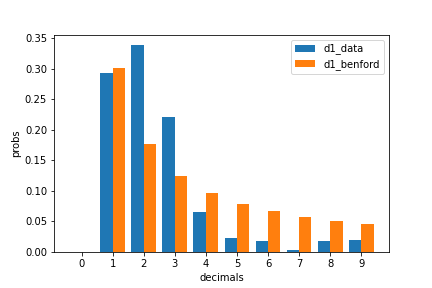
\includegraphics[scale=0.4]{พลงประชารัฐ.png}
  \caption{First Digit Frequency of Palang Pracharat Party}
  \label{fig:sub2}
\end{subfigure}
\caption{First Digit Frequency of all votes and a party}
\label{fig:test}
\end{figure}


\subsection{Chi Square Analysis}
For each party, the chi-square value is calculated as
$$X^2 = \sum_{i=1}^{9}\frac{(O_i - E_i)^2}{E_i}$$ such that $O_i$ is the observed frequency of leading digit $i$ and $E_i$ is the expected frequency of which according to Benford's Law. There are 9 possible first digits; hence, the degree of freedom, which is one less than the number categories, is $8 = 9-1$.

The overall data of the election, counting the votes of all parties (Figure 1), has a chi-square value of $29.65$ and a P-value of $0.0002$, suggesting a non-compliance to Benford's Law statistically at a 95\% confidence level. A similar analysis is further done for each party, among which 57 parties passed the chi-square test (see \href{https://github.com/pond-nj/Benford-s-Law-Analysis/tree/main/thai\%20election\%20graph/p_moreThan0.05}{\textbf{this folder}} for their graphs), while the other 20, with their P-values being less than 0.05, showed non-compliance with Benford's Law. (Their graphs could be found \href{https://github.com/pond-nj/Benford-s-Law-Analysis/tree/main/thai\%20election\%20graph/p_lessThan0.05}{\textbf{here}})

\subsection{Discussion}
\subsubsection* {Why some parties do not comply}
Non-compliance to Benford's Law could indicate a potential fraud. However, interestingly, the mean value of the sample size of 20 parties that do not statistically comply with Benford's Law is $253.8$, while the mean value of those do is $96.75$. Plotting the distribution of sample sizes results in Figure 2.

\begin{figure}[h]
\centering
\begin{subfigure}{.5\textwidth}
  \centering
  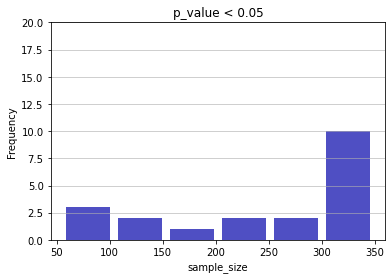
\includegraphics[scale=0.4]{p_value_less.png}
  \caption{p-value less than 0.05}
  \label{fig:sub1}
\end{subfigure}%
\begin{subfigure}{.5\textwidth}
  \centering
  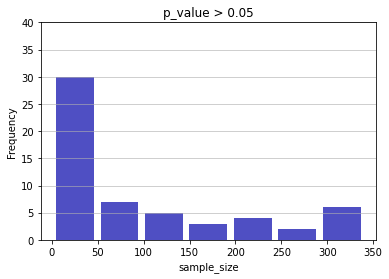
\includegraphics[scale=0.4]{p_value_more.png}
  \caption{p-value more than 0.05}
  \label{fig:sub2}
\end{subfigure}
\caption{Distribution of sample size of parties with p-value with compared to 0.05}
\label{fig:test}
\end{figure}


These figures showed the data with a larger sample size is less likely to comply with Benford's Law compared to those with smaller size, which is heavily counter-intuitive, with the ultimate example that the statistical analysis of the overall data (Figure 1a) also shows a non-compliance to Benford's Law. Therefore, while we could question the use of chi-square test as a statistical test, we suspect that the variability of the data set is instead the culprit.

\subsubsection{The variability of dataset: A Robust Measure of Order of Magnitude}


Variability and spread of a data set should be considered while analysing using Benford's Law. The order of magnitude reflects variability of a data set, and large order of magnitude is essential for such analysis. In order to avoid the influence of outliers and  whiskers, the robust order of magnitude should be considered, according to \cite{alex}, i.e., to focus on the core 98\% part of the data. Take $P_{1\%}$ as the 1st percentile of the data set and $P_{99\%}$ as the 99th percentile of the data set. $$\text{Robust Order of Magnitude (ROM)} = \log_{10}(P_{99\%}/P_{1\%})$$ Ideally, the value of the (robust) order of magnitude of the data set should be more than 3.

As we calculated the robust measure of order of magnitude(ROM) for data sets of all parties, only one has the value of ROM over 3; the voting data of this party complies with Benford’s Law, as the P-value of chi-square is 0.1004, which is above the significance level of 0.05. 

\subsubsection {Questioning the use of chi-square test}
While, we believe the debatable result is a consequence of non-diversified data set. We also question the use of chi-square test. According to \textcite{alex}, chi-square is not a good statistical test for Benford's Law since it has no statistical validity in many real-life data sets. Instead, Sum of Square Deviations (SSD) is recommended to be used \cite{alex}. Therefore, future work could be done comparing the use of SSD test and chi-sqauare test.

\subsection{Future Work}
It is discovered that different base representation of Benford's Distribution also conforms to Benford's Law \cite{SCHATTE1998391}. Thus, work could be done to examine the dataset is other bases. Moreover, second digit analysis could be conducted further to explore the conformity to Benford's Law.

\section{Conclusion}

The overall votes analysis does not fit Benford's Law statistically using the chi-square test, while, when the examination is done on individual parties, 57 parties from 77 parties show positive compliance to Benford's Law. A closer examination of sample size distribution suggests a doubt on the data's order of magnitude, furthermore, we also question the use of chi-square as a statistical test. All in all, it must be noted that Benford's Law analysis does not indicate any fraudulent behaviour directly; the law itself is no more than a tool to identify suspicious entries. Therefore, further case-examination and data analysis must be conducted as discussed.

\medskip

\printbibliography

\end{document}